\pdfminorversion=4
\documentclass[aspectratio=169]{beamer}

\mode<presentation>
{
  \usetheme{default}
  \usecolortheme{default}
  \usefonttheme{default}
  \setbeamertemplate{navigation symbols}{}
  \setbeamertemplate{caption}[numbered]
  \setbeamertemplate{footline}[frame number]  % or "page number"
  \setbeamercolor{frametitle}{fg=white}
  \setbeamercolor{footline}{fg=black}
} 

\usepackage[english]{babel}
\usepackage{inputenc}
\usepackage{tikz}
\usepackage{courier}
\usepackage{array}
\usepackage{bold-extra}
\usepackage{minted}
\usepackage[thicklines]{cancel}
\usepackage{fancyvrb}

\xdefinecolor{dianablue}{rgb}{0.18,0.24,0.31}
\xdefinecolor{darkblue}{rgb}{0.1,0.1,0.7}
\xdefinecolor{darkgreen}{rgb}{0,0.5,0}
\xdefinecolor{darkgrey}{rgb}{0.35,0.35,0.35}
\xdefinecolor{darkorange}{rgb}{0.8,0.5,0}
\xdefinecolor{darkred}{rgb}{0.7,0,0}
\definecolor{darkgreen}{rgb}{0,0.6,0}
\definecolor{mauve}{rgb}{0.58,0,0.82}

\title[2024-12-17-complex-step-autodiff]{Awkward Array's JAX backend and \\ complex-step autodiff as an alternative}
\author{Jim Pivarski}
\institute{Princeton University -- IRIS-HEP}
\date{December 17, 2024}

\usetikzlibrary{shapes.callouts}

\begin{document}

\logo{\pgfputat{\pgfxy(0.11, 7.4)}{\pgfbox[right,base]{\tikz{\filldraw[fill=dianablue, draw=none] (0 cm, 0 cm) rectangle (50 cm, 1 cm);}\mbox{\hspace{-8 cm}
\includegraphics[height=1 cm]{princeton-logo-long.png}\hspace{0.1 cm}\raisebox{0.1 cm}{
\includegraphics[height=0.8 cm]{iris-hep-logo-long.png}}\hspace{0.1 cm}}}}}

\begin{frame}
  \titlepage
\end{frame}

\logo{\pgfputat{\pgfxy(0.11, 7.4)}{\pgfbox[right,base]{\tikz{\filldraw[fill=dianablue, draw=none] (0 cm, 0 cm) rectangle (50 cm, 1 cm);}\mbox{\hspace{-8 cm}
\includegraphics[height=1 cm]{princeton-logo.png}\hspace{0.1 cm}\raisebox{0.1 cm}{
\includegraphics[height=0.8 cm]{iris-hep-logo.png}}\hspace{0.1 cm}}}}}

% Uncomment these lines for an automatically generated outline.
%\begin{frame}{Outline}
%  \tableofcontents
%\end{frame}

% START START START START START START START START START START START START START

\begin{frame}{Awkward Array has 4 backends}
\large
\vspace{0.5 cm}
\begin{itemize}\setlength{\itemsep}{0.5 cm}
\item \mintinline{python}{"cpu"}: buffers (user data, indexes, offsets, etc.) are NumPy arrays, computations are performed by NumPy functions or cpu-kernels.so
\item \mintinline{python}{"cuda"}: buffers are CuPy arrays, CUDA kernels are JIT-compiled by CuPy
\item \mintinline{python}{"typetracer"}: buffers are dataless Python objects that only infer types (intended for Dask; currently only used by Dask)
\item \mintinline{python}{"jax"}: data buffers are JAX arrays, indexes are NumPy, \mintinline{python}{ak.Array} is flattened/unflattened as PyTrees
\end{itemize}

\vspace{0.5 cm}
When a backend is untested, it gets out of date. \mintinline{python}{"jax"} has 44 tests. (\mintinline{python}{"cuda"} has 459 tests and \mintinline{python}{"cpu"} + \mintinline{python}{"typetracer"} has 2214 tests and are used daily.)
\end{frame}

\begin{frame}{JAX backend development}
\large
\vspace{0.5 cm}
\begin{columns}
\column{1.1\linewidth}
\only<1>{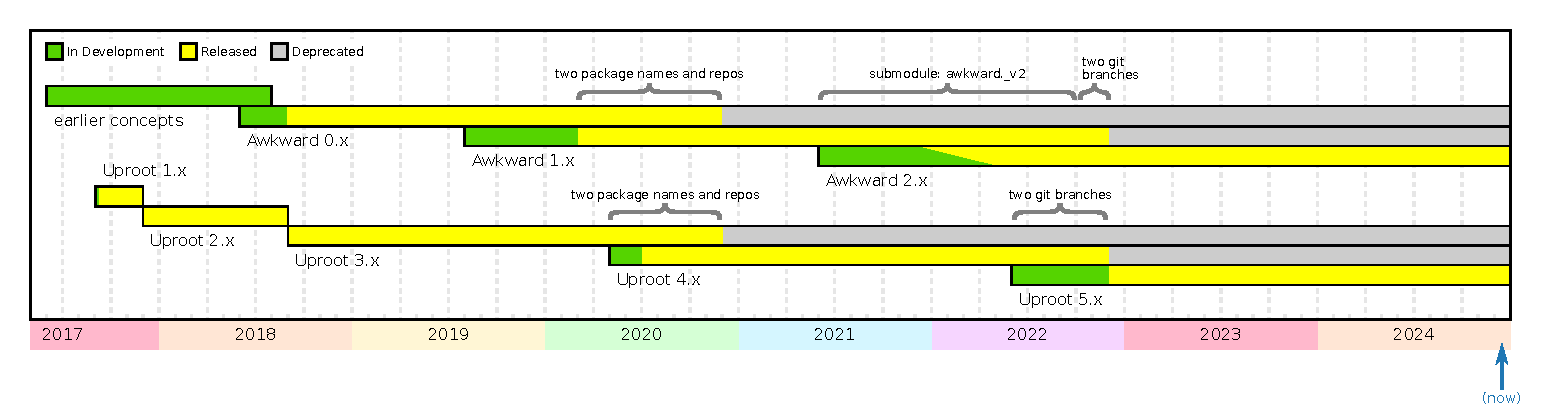
\includegraphics[width=\linewidth]{awkward-uproot-timeline.pdf}}\only<2->{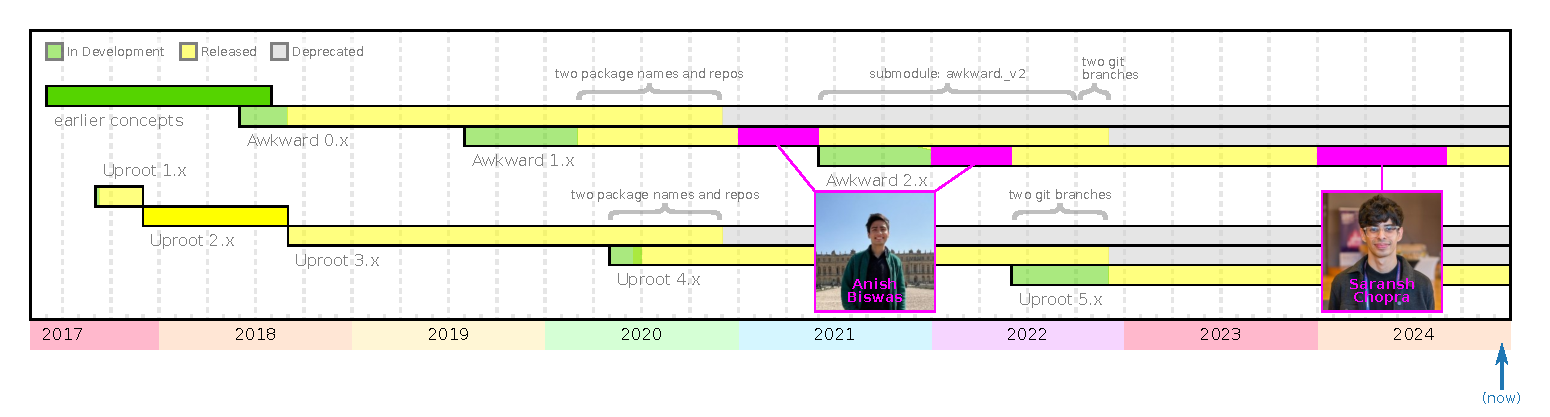
\includegraphics[width=\linewidth]{awkward-uproot-timeline-jax.pdf}}
\end{columns}

\begin{uncoverenv}<2->
\begin{itemize}\setlength{\itemsep}{0.25 cm}
\item Jan 2021--Apr 2021: Anish Biswas as IRIS-HEP Fellow
\begin{itemize}
\item wasn't possible at all, motivated Awkward v2 C++ $\to$ Python reimplementation
\end{itemize}
\item Jan 2022--Jun 2022: Anish Biswas as CERN Contractor
\begin{itemize}
\item implemented map-like functions in PyTrees, reduce-like functions with LAX
\end{itemize}
\item Jan 2024--Sep 2024: Saransh Chopra as IRIS-HEP Gap Year Fellow
\begin{itemize}
\item ``on call'' for feedback from autograd users; received very little
\end{itemize}
\end{itemize}
\end{uncoverenv}
\end{frame}

\begin{frame}{Occasionally, the JAX tests fail and are patched}
\vspace{0.25 cm}
\begin{columns}
\column{0.55\linewidth}
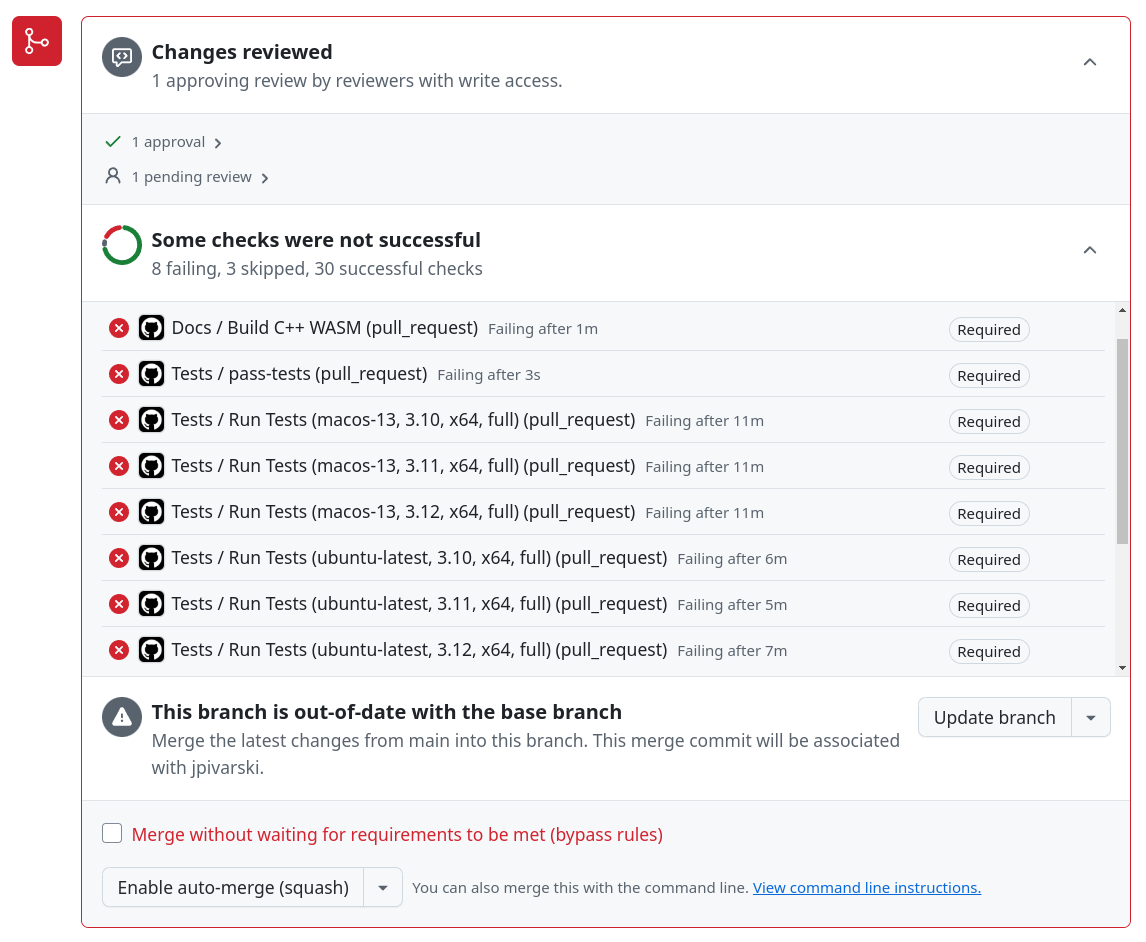
\includegraphics[width=\linewidth]{jax-failures.png}

\column{0.5\linewidth}
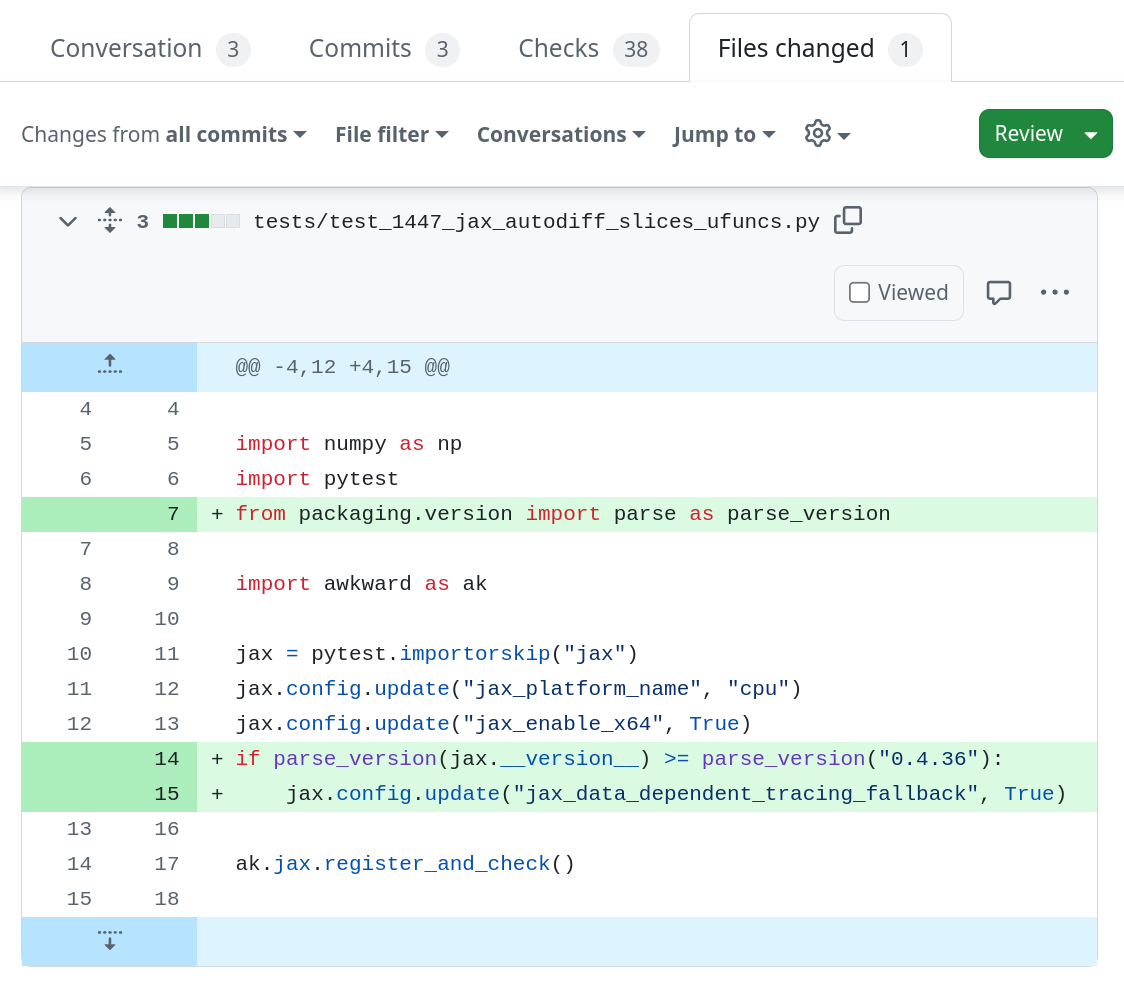
\includegraphics[width=\linewidth]{jax-failures-2.png}
\end{columns}
\end{frame}




\end{document}
